\documentclass[a4paper,10pt]{extarticle}

\usepackage{amsmath}
\usepackage{amssymb}
\usepackage{charter}
\usepackage{color}
\usepackage{comment}
\usepackage{empheq}
\usepackage{fancyhdr}
\usepackage{lastpage}
\usepackage[T1]{fontenc}
\usepackage[top=2cm, bottom=2cm, left=1.5cm, right=1.5cm]{geometry}
\usepackage{graphicx}
\usepackage[utf8]{inputenc}
\usepackage[normalem]{ulem}
\usepackage{setspace}
\usepackage{titlesec}
\usepackage{tikz}
\usetikzlibrary{arrows}
\usetikzlibrary{positioning,decorations.markings}
\usepackage{amsmath}
\usepackage{pdflscape}
\usepackage{prftree}
\usepackage{pdfpages}

\titleformat{\title}
{\color{black}\normalfont\Large\bfseries\centering}
{\color{black}\thesection}{1em}{\hspace{0cm}}

\titleformat{\section}
{\color{black}\normalfont\Large\bfseries\centering}
{\color{black}\thesection}{1em}{\hspace{0cm}}

\titleformat{\subsection}
{\color{black}\normalfont\large\bfseries}
{\color{black}\thesubsection}{1em}{\hspace{.4cm}}

\titleformat{\subsubsection}
{\color{black}\normalfont\normalsize\bfseries}
{\color{black}\thesubsubsection}{1em}{\hspace{.8cm}}

\begin{document}

\pagestyle{fancy}
\renewcommand{\headheight}{24pt}
\lhead{Pavlos Tserevelakis et Raphaël Lutz}
\rhead{\today}

\section*{Trafic au CERN - Cahier des charges}

\subsection*{Modèle}

Nous choisissons d'implémenter un modèle discret du trafic routier, par automate cellulaire. Ce genre de modèle a fait ses preuves, comme présenté par le professeur Bastien Chopard\footnote{\emph{Cellular Automata Simulations of Traffic:
A Model for the City of Geneva}, A. Dupuis et B. Chopard, Networks and Spatial Economics, 3: (2003) 9–21}.

%\subsubsection*{Avantage}

%Ce type de modèle est simple à mettre en place, et les simulations devraient être rapides.

\subsubsection*{Précision}

\paragraph{Spatiale}

La précision spatiale du modèle sera de 7.5 mètres (longueur d'une cellule). Ceci correspond à la longueur moyenne d'un véhicule sur la route.

\paragraph{Temporelle}

Nous n'avons pas encore pu nous arrêter sur une définition temporelle. Celle-ci serait de l'ordre des secondes.

\subsection*{Langage}

Pour sa rapidité et son efficacité, nous allons implémenter ce modèle en C++. Cela nous permettra de faire des simulations aisément, et d'implémenter une interface afin de visualiser le trafic.

\subsection*{Plateforme}

Pour notre travail, nous utiliserons GitHub afin de garder une trace de l'évolution, et pour permettre un échange facile de nos avancées respectives.

\subsection*{Scénarios envisagés}

Voici la liste des différents scénarios que nous envisageons d'essayer :

\begin{itemize}
\item Situation actuelle
\item Ouverture de l'entrée E et du tunnel inter-site
\item Doubler la voix de l'entrée E
\item Changer la séquence des feux à l'entrée B
\item Remplacer le carrefour de l'entrée B par un rond-point
\item Ajouter une déviation pour l'entrée E, surélevée ou souterraine (fig. 1)
\item Report des véhicules
\begin{itemize}
\item de l'entrée E au tunnel inter-site
\item des véhicules individuels aux transports doux
\end{itemize}
\end{itemize}

\begin{figure}[h!]
\begin{center}
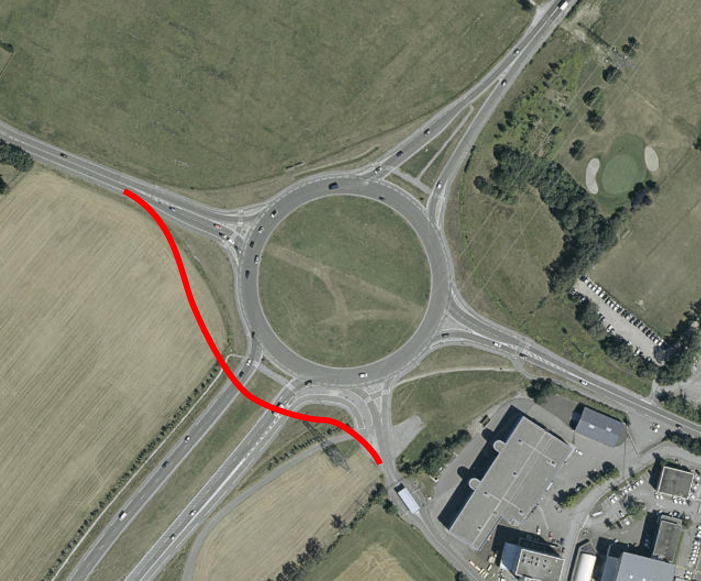
\includegraphics[width=5cm]{plan_E_scenario.png}
\caption{Déviation}
\end{center}
\end{figure}

\subsection*{Calendrier}

Ce calendrier n'est bien évidemment pas définitif. Au fur et à mesure de l'avancée, nous l'adapterons et le mettrons à jour.

\begin{itemize}
\item 27.05 : implémentation du modèle d'automate cellulaire et test pour un segment de route
\item 10.06 : implémentation de rond-points et test
\item 24.06 : implémentation de carrefours/feux et test
\item 08.07 : implémentation d'une interface pour la visualisation du modèle (commencera dès le 27.05)
\item 22.07 : implémentation du réseau routier autours du CERN
\item 05.08 : simulations avec les données mesurées
\item 19.08 : test des scénarios
\end{itemize}


\end{document}
